\documentclass[conference]{IEEEtran}
\makeatletter
\newcommand{\rmnum}[1]{\romannumeral #1}
\newcommand{\Rmnum}[1]{\expandafter\@slowromancap\romannumeral #1@}
\makeatother

\usepackage{epsfig}
\usepackage{amsopn}
\usepackage{subfigure}
\usepackage{cite}
\ifCLASSINFOpdf

\else
\fi
\usepackage[cmex10]{amsmath}

\interdisplaylinepenalty = 2500

\usepackage{algorithmic}
\usepackage{algorithm}
\hyphenation{op-tical net-works semi-conduc-tor}


\begin{document}
\title{Access Strategy in Super WiFi Network Powered by Solar Energy Harvesting, A POMDP Method}

\author{\authorblockN{Tingwu~Wang\authorrefmark{1},
	Chunxiao~Jiang\authorrefmark{1},
	Yan~Chen\authorrefmark{2},
	Yong~Ren\authorrefmark{1}, and
	K. J. Ray~Liu\authorrefmark{2}}
	\small\authorblockA{\authorrefmark{1}
		Department of Electronic Engineering, Tsinghua University, Beijing, 100084, P. R. China\\
          \authorrefmark{2}Department of Electrical and Computer Engineering,
		  University of Maryland, College Park, MD 20742, USA\\
        E-mail: wtw12@mails.tsinghua.edu.cn, \{jchx, reny\}@tsinghua.edu.cn, \{yan, kjrliu\}@umd.edu}}
\maketitle

\begin{abstract}
The recently announced Super Wi-Fi Network proposal is aiming to enable Internet access in a nation-wide area.
As traditional cable-connected power supply system becomes impractical or costly for a wide range wireless network,
new infrastructure deployment for Super Wi-Fi is needed.
The fast developing Energy Harvesting (EH) techniques receive global 
concerns for their potential of solving the above power supply problem. 
Many studies have been done on traditional access strategy,
but the access strategy in EH wireless network with multiple Base Stations (BS)
remains a field with tremendous research potential.
Different from traditional wireless network,
a Base Station (BS) in EH powered network harvests energy from the ambient environment.
And as the energy is limited, 
the BS will not broadcast its system state to all the users within its range,
which provides incomplete information for the users. 
Thus the access strategy has to be carefully chosen.
In this paper, we propose a practical and efficient framework for multiple BSs access strategy
in an EH powered Super Wi-Fi network.
In our work, we consider the access strategy from the a user perspective,
who exploits downlink transmission opportunities from BS.
To formulate the problem,
we used Partially Observable Markov Decision Process (POMDP) to model the
real world uncertainty.
Simulation results show that our methods are efficacious and significantly outperforms
the traditional widely used CSMA method.
\end{abstract}
\IEEEpeerreviewmaketitle
\section{Introduction}
% ------------------------------------------------------------------------------------------- %
% background
In order to expand the coverage area of wireless network,
many algorithms and implementations have been revised.
And recently, the Federal Communications Commission published the Super Wi-Fi proposal,
aiming to make use of lower-frequency white spaces between television channel frequencies
and create a nationwide wireless network.
However, the ambitious task of building a countrywide network comes across many obstacles.
An inevitable problem is how to deploy practical backhaul and energy supply system.
Traditional cable-based systems are excessive, considering the cost for deploying and maintaining the network,
and sometimes impossible as well as dangerous in complex environment.
Despite all the above difficulties, there are solutions and
many successful experimental deployments of Super Wi-Fi are accomplished accordingly.
Wireless backhual has been proven to be effective \cite{30} as a replacement for cable backhaul.
And the fast developing EH technology provides an ideal replacement as the power supply problem, 
which could make use of a wide range of ambient energy including piezoelectric, thermal, solar energy, etc.\\
% ------------------------------------------------------------------------------------------- %
% previous work
\indent As the deployment of EH network is just emerging,
new wireless protocols and modification are needed, as some preliminary studies pointed out \cite{27}.
Previously, the access strategy problem has been a core problem in wireless communications,
and many researchers have been doing some brilliant work in the literature.
Markov Decision Process have been widely used in wireless network,
with some challenges and solutions summarized in \cite{23}.
Access process is a typical game process,
and therefore game theory, summarized in \cite{22},
and pricing theory, used in \cite{7}, has been applied respectively.
In \cite{5}, the access strategy towards multiple BSs with negative externality is considered.
More recently, a POMDP MAC layer opportunistic access is proposed by Dr. Zhao in \cite{zhao1}.
A learning based approach to access between packet bursts is studied in \cite{kae1}.
\\
% ------------------------------------------------------------------------------------------- %
% our work
\indent However, all the mentioned existing studies on the access strategy did not consider the 
multiple BSs access strategy under energy harvesting, while, as mentioned above,
using EH powered BSs is the best practicable ways of realizing Super Wi-Fi network.
In this work, we propose an access strategy that is exercisable in the fast booming Super Wi-Fi network.
The special characteristics and their adjoint problems in the EH powered network are studied and solved.
As long time transmission is not guaranteed in EH network,
leaving and arriving of users is more frequent.
Instead of using a static system model,
we consider a model where the number of accessing users and the battery are dynamic.
A revised birth and death process and a battery transition formulation based on quasi-static assumption
are combined to describe system state transition.
Besides, unlike most of the models where the strategy of the users on the BSs is neglected,
we consider the case where an user's decision affects system state.
It is more rational than previous models with no affection.
As, for example, in EH powered network, a user could cause energy depletion,
collision and system low efficiency if it performs short-sighted and selfish strategy,
or causing energy waste when it is too conservative.
And as in EH wireless network, the full knowledge of the system is unrealistic,
a POMDP model is used to formulate the problem, where the information of the system is obtained by observations.
% conclusion about our model
To sum up, we propose an algorithm that is able to overcome the shortcomings in previous models.
And although our work focuses on solar energy harvesting,
it is clear that the conclusion and the algorithm could be generalized to any access problems in EH powered network.
\\
% ------------------------------------------------------------------------------------------- %
% organization
\indent The rest of this paper is organized as follow.
We describe the system model In Section \Rmnum{2}.
And in Section \Rmnum{3}, the POMDP access strategy is presented,
showing how we formulate the continuous battery state and user state to
POMDP states and obtain the optimal decision. And a suboptimal strategy is proposed.
In Section \Rmnum{4}, we evaluate the performance of our proposed approach with several famous traditional algorithm.
Finally, Section \Rmnum{5} draws the conclusion.
% ------------------------------------------------------------------------------------------- %
% ----------------------------end of introduction-------------------------------------------- %
% ------------------------------------------------------------------------------------------- %
\begin{figure}\label{fig1}
\centering
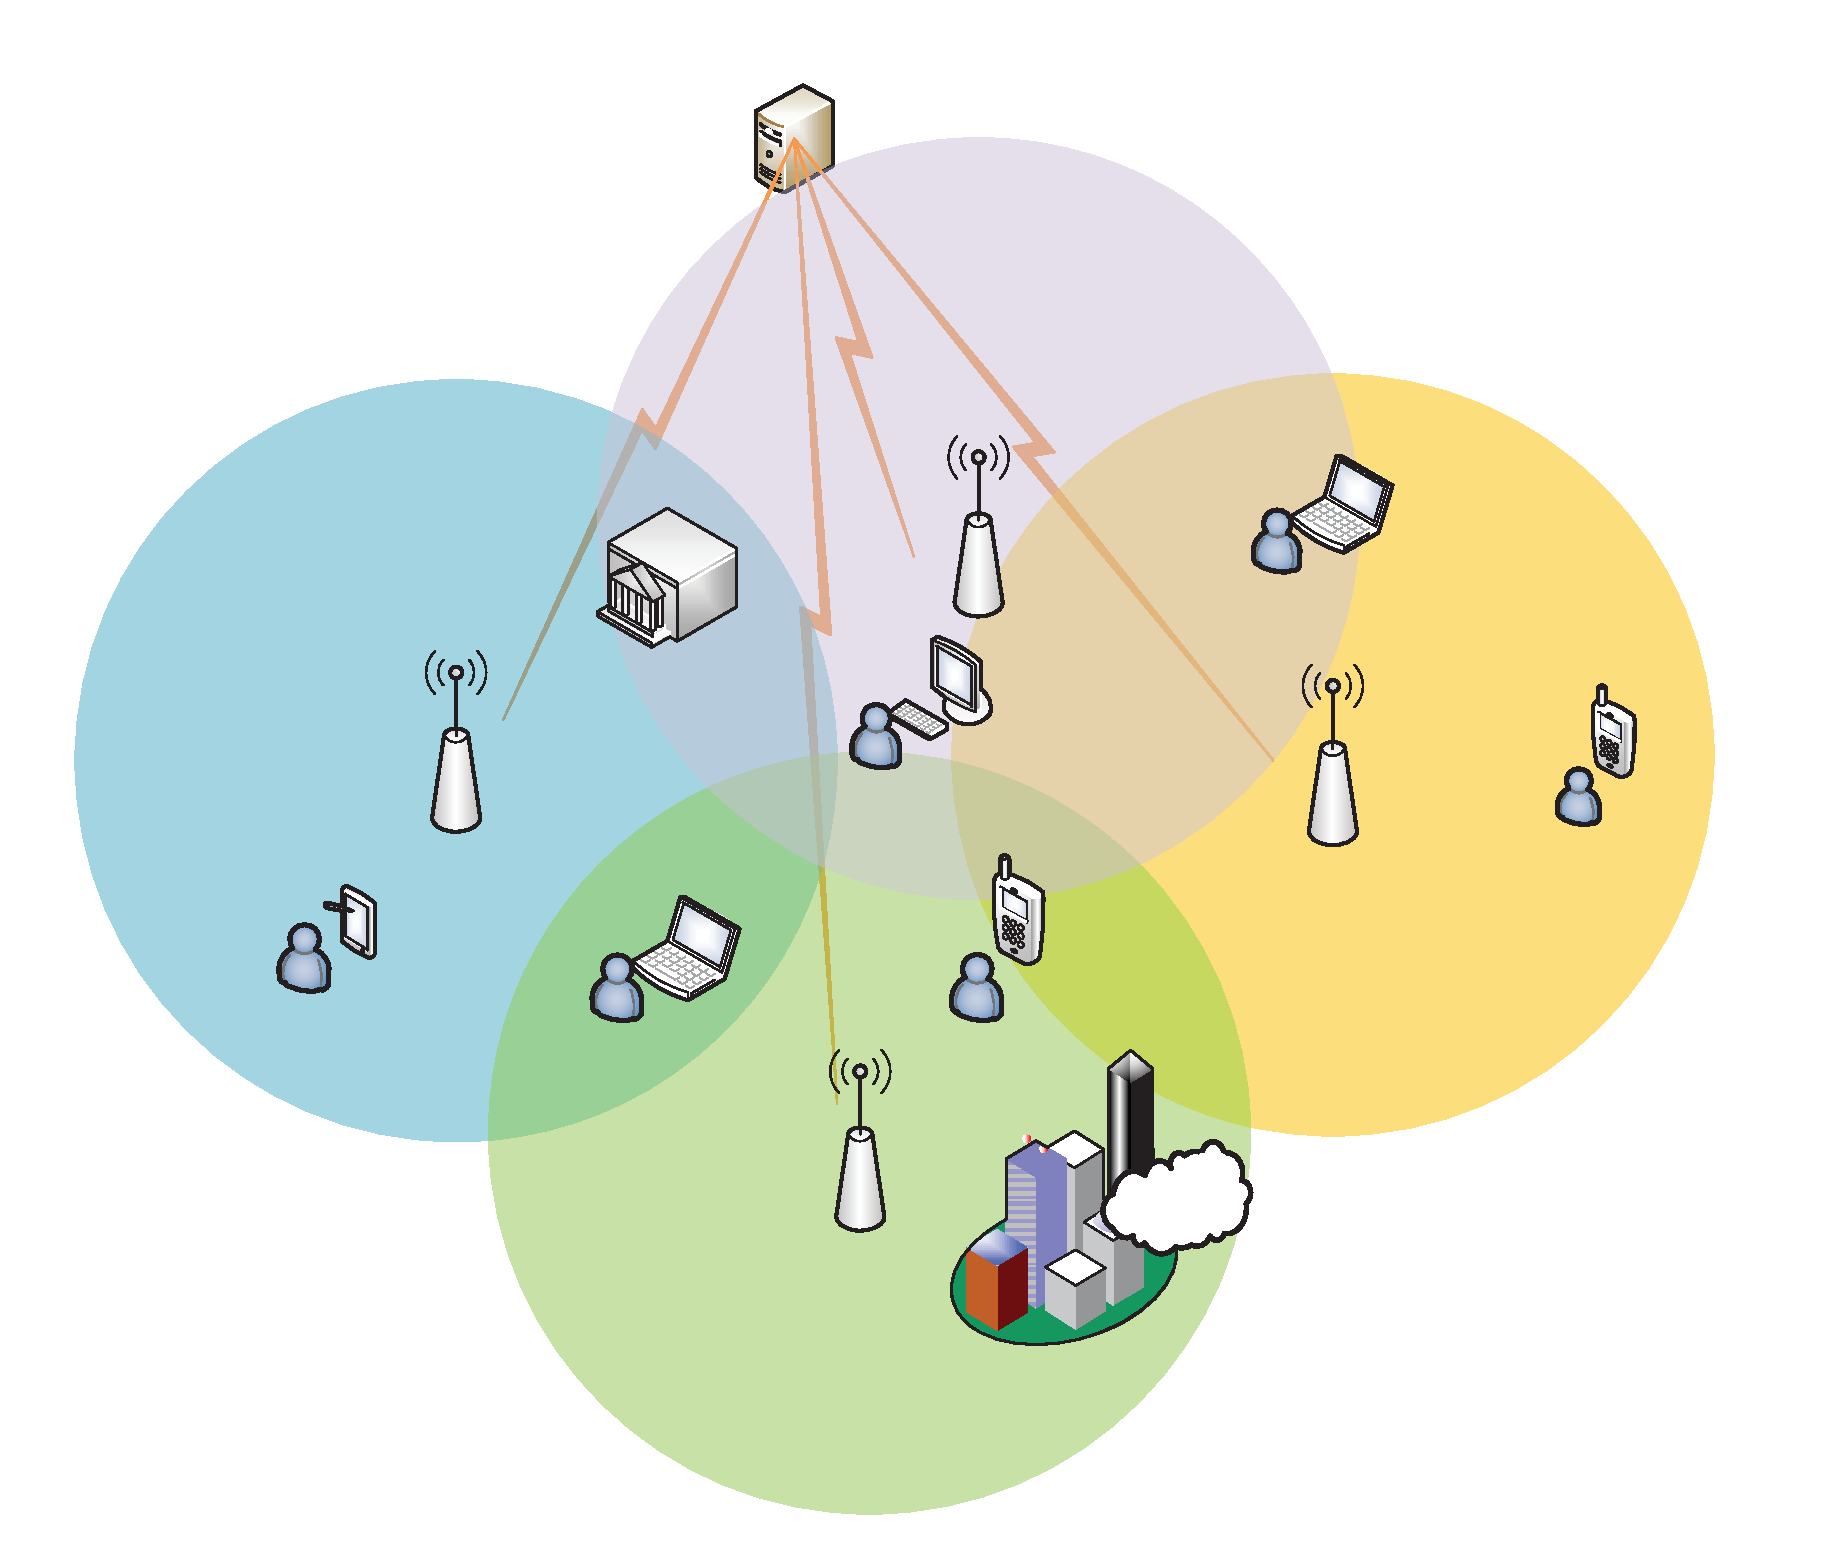
\includegraphics[width=8.5cm]{Fig1.eps}
\caption{A schematic map of Super Wi-Fi system.}
\end{figure}
\section{System Model}
In this section, we describe the system model of the Super Wi-Fi EH network.
As shown in Fig. 1, in an EH network, there are multiple BSs. 
And like traditional wireless network, the users arrive and leave the BS with certain probability \cite{5}.
In our work, we consider a rational user who could observe multiple BSs and
choose an action in every time slot to maximize its utility.
We denote the number of observed BSs by the user as \(N_A\).
The BSs have a maximum number of users to serve simultaneously due to limited spectrum and coding ability.
We use the notation \(N_U\) to represent the maximum number of users.
Thus, the user state in each BS could be denoted as \(S_U = i,\, i = \,0,\,1,\,\ldots,\,N_U-1\).
Besides, each BS has a limited and changing battery quantity,
which could be any continuous value between \(0\) and the maximum battery value \(B_M\).
Note that in our work, the \(B_M\) and \(N_U\) for different BSs could be different and our method still works.\\
\subsection{User Model}
During each time slot, a certain quantity of energy, denoted as \(E_H\) is harvested from external environment.
And at the same time, a quantity of energy \(E_T\) is consumed for transmitting wireless signal.
Between adjacent time slots, new users may arrive and
old users may actively leave or forced be forced to leave when battery is not adequate.
And in order to model the forced leaving phenomenon,
we revise the birth and death process to describe user behaviors.
The transition probability of user number is calculated as,
\begin{align}\label{formula1}
&\zeta\left(S_U'| S_U, Q_B, \Phi\right) = \nonumber\\
&\begin{cases}
	\lambda, &\mbox{if $Q_B$ is enough and $S_U' = S_U + 1$,}\\
	\mu S_U, &\mbox{if $Q_B$ is enough and $S_U' = S_U - 1$,}\\
	I_0\left(S_U'\right), &\mbox{if $Q_B$ is insufficient,}\\
	0, &\mbox{otherwise.}\\
\end{cases}
\end{align}
In the above equation, \(\lambda\) is the arriving rate and
the \(\mu' = \mu S_U\) is the leaving rate of birth and death process.
Note that when the battery is exhausted, all the users are forced to leave,
which is represented by the indicator function \(I_0\left(S_U'\right)\),
i.e., \(S_U'\) is sure to be \(0\) next time slot.
When the battery is not enough, we have \(Q_B- E_T \leq 0\), 
and the BS sends signal to inform that the battery is using up and users have to leave.
\subsection{Access Model and Observation Model}
At the start of each time slot,
to maximize utility, the rational user could either access or sense one of the BSs within its range.
We denote the action as \(\Phi = \Phi_{a}^i\) for accessing the \(i^{th}\) BS,
and \(\Phi = \Phi_{s}^i\) for sensing.
In the case of accessing, the user sends a request signal to the chosen BS.
When request is achievable, BS will activate user's transmission immediately.
When request is unavailable, the BS will decline the request and
inform the user its system state with a short signal.

When collision happens, the energy is wasted due to low SINR.
% and send back a short message informing the BS of the BS's system state.
In order save time and energy, a more conservative idea is to sense the BS, i.e. \(\Phi_{s}^i\).
When the BS receives a sense signal,
it only transmits its system state to the user with neglectable energy consumption.
\subsection{Physical Battery Model}
The harvested energy \(E_T\) is determined by the environmental parameters,
which, in our case, is the sun light intensity.
Gaussian model has been proved effective in predicting sun light intensity \cite{gaussian,data}.
In a small time slot, denoted as \(T_L\), the average solar intensity remains unchanged.
In our work, the solar intensity \(W_e\) is assumed to be
Gaussian distributed with average intensity \(\mu_S\) and variation \(\sigma_S\), \(\mathcal{N}\left(x;\mu_S,\sigma_S\right)\).
The harvested energy is given as \(E_H = W_eJ_{op}V_{op}\Omega_ST_L\eta\),
where the \(J_{op}\) and \(V_{op}\) is the optimal operating point of the existing harvesting devices \cite{physic},
the \(\Omega_S\) is the number of solar cells and the \(\eta\) is the harvesting efficiency.
The transmitting energy is adjusted to make sure transmission with certain SINR.
It is important to note that, current feedback-based power adjustment algorithm
like Inner Loop Power Management is not valid as the system state changes during the time slots.
Here a static power management is implemented.
The power consumption in a BS is determined by number of users and the current user' action,
which is \(E_T = \Upsilon_T(S_U, Q_B, \Phi)\).
The access of our user could be regarded as an extra ordinary user for the BS, i.e., for BS \(i\),
\(\Upsilon_T(S_U, Q_B, \Phi = \Phi_{a}^{i}) = \Upsilon_T(S_U + 1, Q_B, \Phi \ne \Phi_{a}^i)\).
When the required battery is more than the BS's remaining battery,
the users with the higher priority is served.
In our case, the opportunistic user we consider has the lowest priority.
Now we could define the event that \(Q_B\) is adequate as \(Q_B- \Upsilon_T(S_U, Q_B, \Phi) \leq 0\).
Thus the battery in the next time slot could be expressed as follow,
\begin{equation}
	Q_B' = \mbox{min}\{Q_B + E_H - E_T, B_M\}.
\end{equation}
To protect passive users from our opportunistic user who could
uses up all the energy, our user will not be served by BS in shortage of energy,
for example, BS with energy for only serving one user in one time slot.
\section{POMDP AP selection}
In Section \Rmnum{2} we describe the system model, it is clear that decision has to be carefully chosen.
There are several factors to be considered: the tradeoff between immediate reward and the long term reward and
the uncertainty of system state during decision making.
POMDP, which is recently developing as a strong tool to deal with decision making under uncertainty,
come as a perfect solution to this system.
However, before we could formulate our proposed algorithm, it is important to define our system state.
\subsection{Battery Transition}
In the implementation of EH powered BSs, the battery is a continuous value.
And in a POMDP, the states have to discrete.
Intuitively, we could use more battery states to represent the same battery volume,
but this brings much increase in the complexity of POMDP.
In our work, we convert the continuous battery quantity into \(N_B\) discrete battery states
\(S_B = \lfloor Q_B N_B / B_M \rfloor\). \(S_B\) could take values from level \(0,\,1,\,\ldots,\,N_B - 1\).
In order to calculate the transition probability between adjacent battery states,
we assume the fluctuate of discrete battery state is quasi-static.
Under the assumption, for a given discrete battery state \(S_B\),
the residue energy \(Q_B - B_MS_B/N_B\) is uniformly distributed between \(\lbrack0,\,B_M/N_B\rbrack\).
Clearly errors are brought by this assumption,
but the quasi-static assumption is proven to be effective
and works well after many time slots \cite{data}.
We denote the battery state changing between time slot as \(\Delta_B = S_{B}' - S_B\).
We define a event \(\xi_j\) to denote that the real battery quantity change is more than \(j\) but less than \(j+1\) levels.
\(\xi_j := \{j\leq N_B\frac{E_H - E_T}{B_M} \le j+1\}\)
Then the probability could be computed as follow,
\begin{align}&\mbox{Pr}\left(\Delta_B = i |\Phi, E_H, \xi_j \right)\nonumber\\
=&\begin{cases} N_B\frac{\left(E_H - E_T\right)}{B_M} -j, &\mbox{$i = j + 1$},\\
\left(j+1\right) -N_B\frac{\left(E_H - E_T\right)} {B_M}, &\mbox{$i = j$},\\
0, &\mbox{otherwise.}\\
\end{cases}
\end{align}
In the equation, as mentioned in previous section, \(E_T = \Upsilon_T(S_U, Q_B, \Phi)\).
The situation where the \(E_H - E_T \le 0\) is simply doing the mirror computation of the above equation.
When we consider the Gaussian distributed light density, the actual battery transition is then,
\begin{equation}\label{battery}
\begin{aligned}
	&\mbox{Pr}\left(\Delta_B = i |\Phi\right) = \\
	&\int_{\frac{iB_M}{N_B} + E_T}^{\frac{\left(i+1\right)B_M}{N_B} + E_T}
	\mbox{Pr}\left(\Delta_B = i |\Phi, E_H, \xi_i\right) \mathcal{N}\left(E_H;\bar{\mu_S},\bar{\sigma_S}\right) dE_H+\\
	& \int_{\frac{\left(i-1\right)B_M}{N_B} + E_T}^{\frac{iB_M}{N_B} + E_T}
	\mbox{Pr}\left(\Delta_B = i |\Phi, E_H, \xi_{i-1}\right) \mathcal{N}\left(E_H;\bar{\mu_S},\bar{\sigma_S}\right) dE_H.\\
\end{aligned}
\end{equation}
In the equation, the mean and variance of the Gaussian distribution are scaled accordingly after mutiplication.
\subsection{System Transition Probability}
When the user transition probability and battery transition probability is computable,
we could focus on the formulation of POMDP.
Note that the POMDP state is the system state, which contains state information of all BS.
To make the following math more readable and flexible,
two equivalent notation of system state is used simultaneously, i.e.
the centralized form of system state \(S\) and
the decentralized form of system state \(S_D = \{S_B^1,\,S_U^1,\,\ldots,\,S_B^{N_A},\,S_U^{N_A}\}\).
\(S = 1,\,2,\, \ldots\,N_S\), where \(N_S = \left(N_BN_U\right)^{N_A}\) is the number of system state.
For the transition probability for a single BS,
the probability of \(S_U'\) and \(S_B'\) in the next slot are conditionally independent
given the current \(S_U\), \(S_B\) and \(\Phi\).
\begin{equation}
\begin{aligned}
	\mbox{P}\left(S_U',S_B'|S_U,S_B,\Phi\right) =
	\zeta\left(S_U'|S_U, S_B, \Phi\right) \delta\left(S_B'|S_U, S_B, \Phi\right).\\
\end{aligned}
\end{equation}
The \(\zeta\left(S_U'|S_U, S_B, \Phi\right)\) is given in equation \eqref{formula1}.
And the battery transition is calculated based on the equation \eqref{battery},
\begin{align}
	&\delta\left(S_B'|S_U, S_B, \Phi\right)\nonumber\\
	= &
	\begin{cases}
		\mbox{Pr}\left(\Delta_B = S_B' - S_B|\Phi \right), &\mbox{if $S_B' \le N_B - 1$,}\\
		\sum_{\Delta_B = S_B' - S_B}^{\Delta_B = \Delta_B^{Max}}\mbox{Pr}\left(\Delta_B|\Phi\right),
		&\mbox{if $S_B' = N_B - 1$.}\\
\end{cases}
\end{align}
In the case of battery overflow, \(S_B'=N_B - 1\), all the extra battery is abondoned.
We truncate the probability above \(\Delta_B^{Max}\) as they are as small as zero by \(4\) decimals.
The overall transition is computed as,
\begin{align}\label{transition}
	T\left(S'|S,\Phi\right) = \prod_{i = 1}^{i = N_A}\mbox{P}\left(S_B^{i,'}, S_U^{i,'}|S_U^i, S_B^i, \Phi\right).
\end{align}
\subsection{POMDP Optimal Algorithm}
In POMDP formulation, the user only has the partial knowledge of the system.
At the end of each slot, the user could get the BS's system state \(S_B^O\) and \(S_U^O\),
which we use \(\mathcal{O}\) to denote.
The observation probability function is given as follow.
\begin{align}
	Z\left(O|S',\Phi\right) = \mbox{Pr}\left(O|S_U^{t,'}, S_B^{t,'}\right) =
	I_{S_U^{t,'},S_B^{t,'}}\left(S_B^O, S_U^O\right).
\end{align}
\(S_B^{t,'}\) and \(S_U^{t,'}\) are the system state of the target BS next time slot.
The indicator function is either \(1\) or \(0\).
The reward is define as \(R = 1\) if the access succeeds, else \(R= 0\).
Then the value function of a single state is,
\begin{equation}
\begin{aligned}
	V_t^\Phi\left(S\right) = R\left(S,\Phi\right) +\gamma\sum\limits_{S'}T\left(S'|S,\Phi\right)V_{t-1}^\pi\left(S'\right),
\end{aligned}%\sum\limits_{O'}Z\left(O|S',\Phi\right)
\end{equation}
where \(\pi\) denotes the optimal action in that state.
As no full knowledge is held for the user, we use a belief vector to denote the system belief
\(\beta = \lbrack \beta\left(S = 1\right),\,\beta\left(S = 2\right),\,\ldots,\,\beta\left(S = N_S\right)\rbrack\).	
Then the particular policy tree with a certain belief \(\beta\) is given as
\begin{equation}
\begin{aligned}
	V_t^\Phi\left(\beta\right) = & \sum\limits_{S}R\left(S,\Phi\right)\beta\left(S\right) +\\
	&	\gamma\sum\limits_{S}\sum\limits_{S'}\beta\left(S\right)T\left(S'|S,\Phi\right)V_{t-1}^\pi\left(S\right).
\end{aligned}
\end{equation}
For simplicity, if we already know all the value function of at the time \(t-1\) during iterations,
a value vector \(\alpha_t^\Phi = \lbrack \alpha_t^\Phi\left(S = 1\right),\,
\alpha_t^\Phi\left(S = 2\right),\,\ldots,\,\alpha_t^\Phi\left(S = N_S\right)\rbrack\)
could be used to simplify the value function as,
\(V_t^\Phi\left(\beta\right) = \sum\beta\left(S\right)\alpha_t^\Phi\left(S\right)\).
Note that for the same \(\Phi\) and \(t\), there are multiple possible \(\alpha\) vectors.
and the optimal action is
\begin{equation}
\begin{aligned}
	\pi\left(\beta\right) =
	\arg\underset{\alpha_t^\Phi}{\max}\sum\limits_{S}\beta\left(S\right)\alpha_t^\Phi.\\
\end{aligned}
\end{equation}
The corresponding value function could be calculated under action \(\pi\left(\beta\right)\).
However, the corresponding optimal policy is not as easy as it seems to be, as the \(\beta\) has a continous value.
But fortunately, note that the \(V_t\) could be regarded as the function value of \(\beta\) in a hyper coordinate,
the axis of which is the components of \(\beta\).
As each set of \(\alpha_t\) vector could be regarded as a set of parameters of a hyper linear function,
% the function value \(V_t\) is piecewise linear with the \(\beta_t\),
there is a dominated hyperplane structure in the model.
The continuous belief space is divided into several \(\alpha\)-vector-dominated hyperplanes.
The partition of belief space in time \(t\) could be calculated given all the dominating \(\alpha_{t-1}\).
The details of algorithm for solving the partition could be find in a well written tutorial \cite{pomdptool}.
At the end of the time slot, the user will update its belief vector according to its observation.
\begin{align}
	\beta'\left(S'|\Phi, O\right) = \frac{\sum_{O}Z\left(O|S',\Phi\right)\sum_{S}
	T\left(S'|S,\Phi\right)\beta\left(S\right)}
	{\sum_{S'}\sum_{O}Z\left(O|S',\Phi\right)\sum_{S}T\left(S'|S,\Phi\right)\beta\left(S\right)}.
\end{align}
\subsection{Suboptimal Access Policy}
The optimal POMDP solution could be calculated off-line within seconds when the number of states is small.
However, the use of POMDP method is limited when \(N_A\) is massive,
and when the environment parameters, like solar coefficients \(\mu_S\), \(\sigma\),
the birth rate \(\lambda\) and death rate \(\mu\) of users, changes quickly.\\
The POMDP formulation tries to maximize success access ration \(\eta_A = N_S/N_T\),
where \(N_S\) is number of success access and \(N_T\) is the number of all the time slots.
We propose a dual perspective of solving the problem, by focusing on the harvested energy.
We name it Energy Based (EB) Method.
The problem is reformulated as,
\begin{equation}
\begin{aligned}
	\underset{\Phi_t,t=0,\,\ldots,\,N_T}{\max}\sum\nolimits_{t=1}^{N_T}
	\mbox{E}\lbrack\mbox{H}\left(\beta^T, \Phi_t\right)\rbrack,\\
\end{aligned}
\end{equation}
where the \(\mbox{H}\left(S^T, \Phi_T\right) = \sum\mbox{min}\left(E_H,\,E_T+B_M-Q_B\right)\)
is the overall harvesting energy of all the BSs combined.
Now a suboptimal could be proposed by maximizing the system's next-time-slot harvested energy.
\begin{equation}
\begin{aligned}
	\Phi_t\left(\beta\right) = \arg{\max}\,\,\mbox{E}\lbrack\mbox{H}(\beta^{t+1}, \Phi_t)\rbrack,\\
\end{aligned}
\end{equation}
When sense is the best action, the user will choose to sense the BS that is not sensed for the longest time.
Due to the limited space, some key rationality of the EB method is summarized.
First of all, when the solar intensity is strong,
we could assume few users will be forced to leave the BS earlier because of a opportunistic user.
And in most cases, the transmitting power \(E_T = \Upsilon_T(S_U, Q_B, \Phi)\).
Thus the reward will increase linearly with the harvested energy.
Second, the EB method is a unselfish method, which would sacrifice some reward,
but will protect overall utility.
Third, the EB method could implement learning algorithm and adjust to quick changes of the environmental parameters,
which will be show in the journal version of this work.
\begin{figure}
\centering
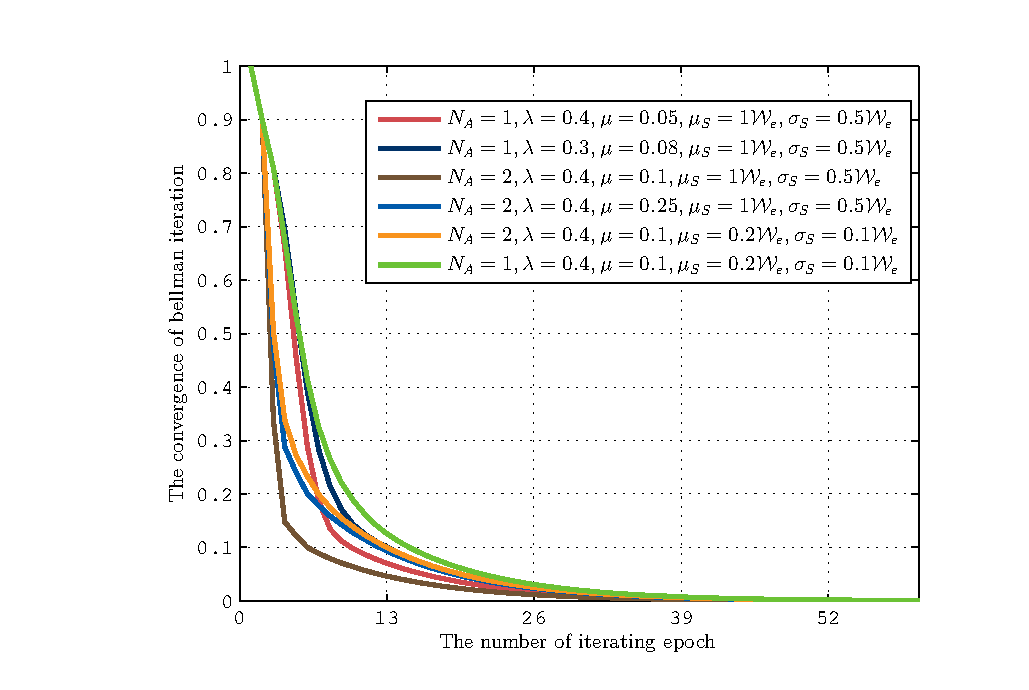
\includegraphics[width=8.5cm]{2_fig3.eps}
\caption{Illustration of the convergence of the POMDP iteration algorithm}
\end{figure}
\section{Simulation Results}
In this section, the convergence and effectiveness of the algorithm is illustrated.
In Fig.2, the convergence of the POMDP iteration algorithm is shown, where discount factor \(\gamma = 0.9\).
A bellman stoping criteria is used to determine the iteration stop.
In the figure the \(\alpha\) vector error shows the convergence of the iteration algorithm.
The POMDP simulation tool is provided by \cite{pomdptool}.
As is clear in the fig, the algorithm converges exponentially.\\
% ------------------------------------------%
\indent The effectiveness of the algorithm is calculated by comparing the \(\eta_A\)
during the overall time slots \(N_T = 10000\).
In the simulation, we use the parameters as follow.
The reference benchmark solar intensity is given as \(\mathcal{W}_e = 1\mbox{kW}/m^2\),
which is the average intensity on the surface of Earth\cite{electric}.
We use the work from \cite{circuit}, where the optimal power per benchmark solar intensity \(\mathcal{W}_e\)
is \(P_H = J_{op}V_{op} = 1.32\mbox{mW}/\mathcal{W}_e\), with a efficiency \(\eta = 75 \%\).
And there are \(\Omega_S = 40\) cells in one harvesting device.
The time slot length is \(T_L = 200\mbox{ms}\).
And as there is no corresponding industry implementation,
we assume a transmission power strategy \(E_T = \Upsilon_T(S_U, Q_B, \Phi)\)
that is proportional to the number of serving users,
which is rational considering a wide range wireless network with negligible between-user interference.
Transmission power for each user is \(P_T = 40\mbox{mW}\).\\
\indent In order to show the efficiency, several algorithms are implemented as comparisons.
CSMA/CA and CSMA/CD methods are used.
Slightly different to the standard CSMA, the users sense the BSs instead of carrier.
And the algorithm tries to avoid collision and energy exhaust.
The CD method will stop request when failure detected. A exponential back-off algorithm is used.
After \(c\) failure, a random number of sleeping time slot between \(0\) and \(2^c - 1\) is chosen.
The CA method will only access after the user sense the BS and know that a successful service is available.
In random access algorithm, the user simply chooses action with equal possibility.\\
\begin{figure}[t]
\centering
\subfigure[The utility ratio with arrival rate in single BS]{
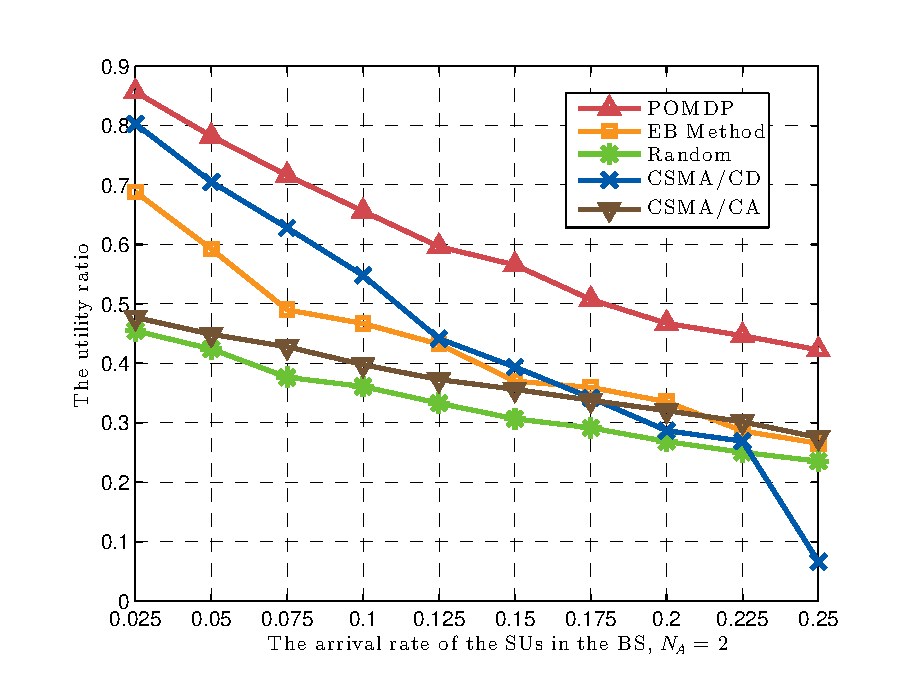
\includegraphics[width=0.5\textwidth]{3_fig1_1.eps}}
\subfigure[The utility ratio with solar intensity in single BS]{
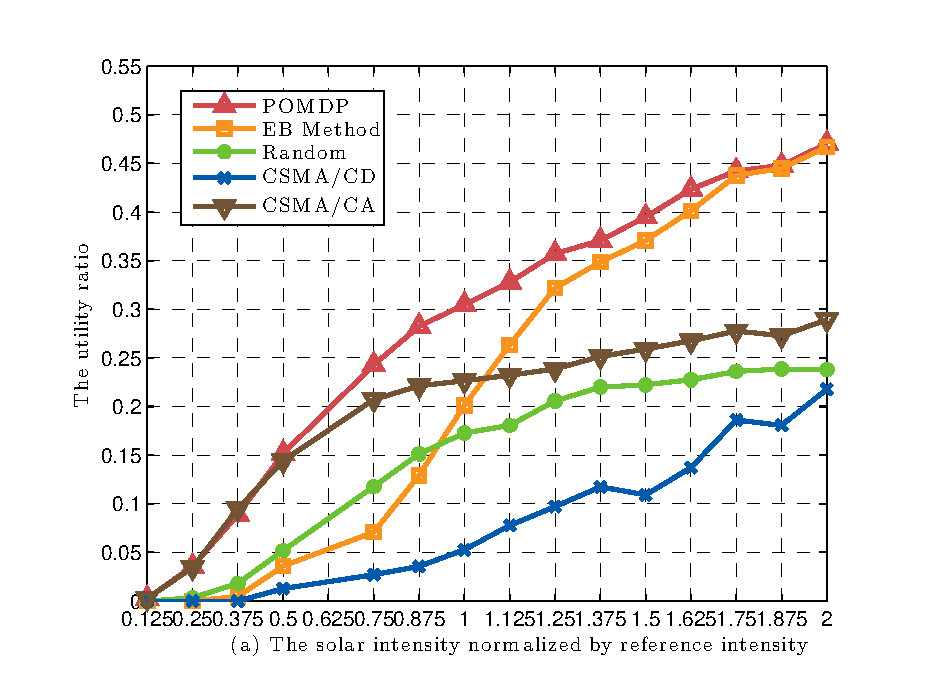
\includegraphics[width=0.5\textwidth]{3_fig2_2.eps}}
\caption{Single BS with \(S_U = 0,\,1,\,2,\,3,\, N_B = 8\)}
\end{figure}
\begin{figure}[t]
\centering
\subfigure[The utility ratio with arrival rate in two BS]{
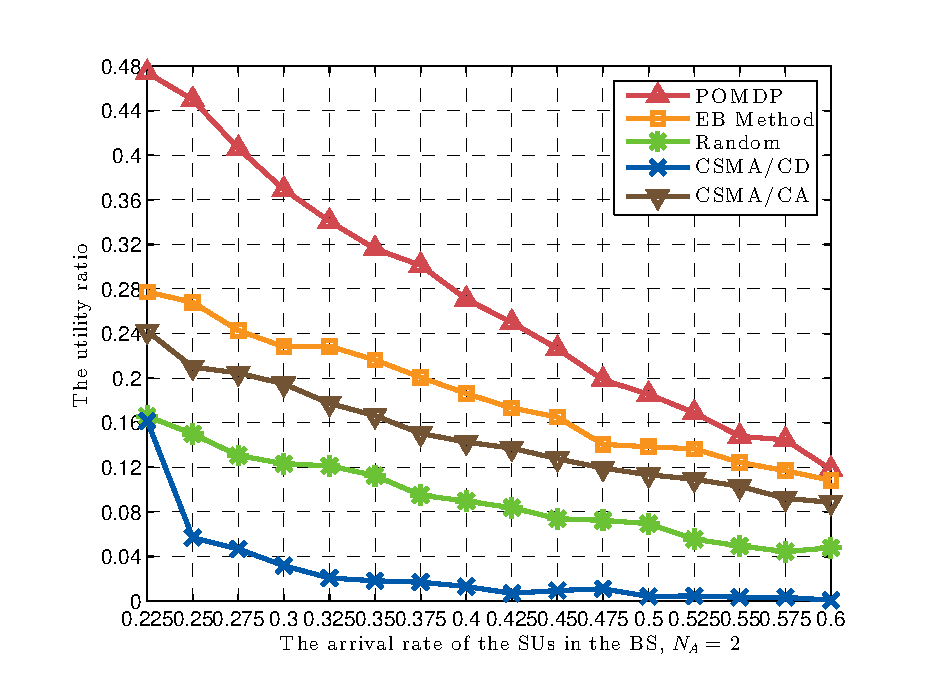
\includegraphics[width=0.5\textwidth]{3_fig2_1.eps}}
\subfigure[The utility ratio with solar intensity in two BS]{
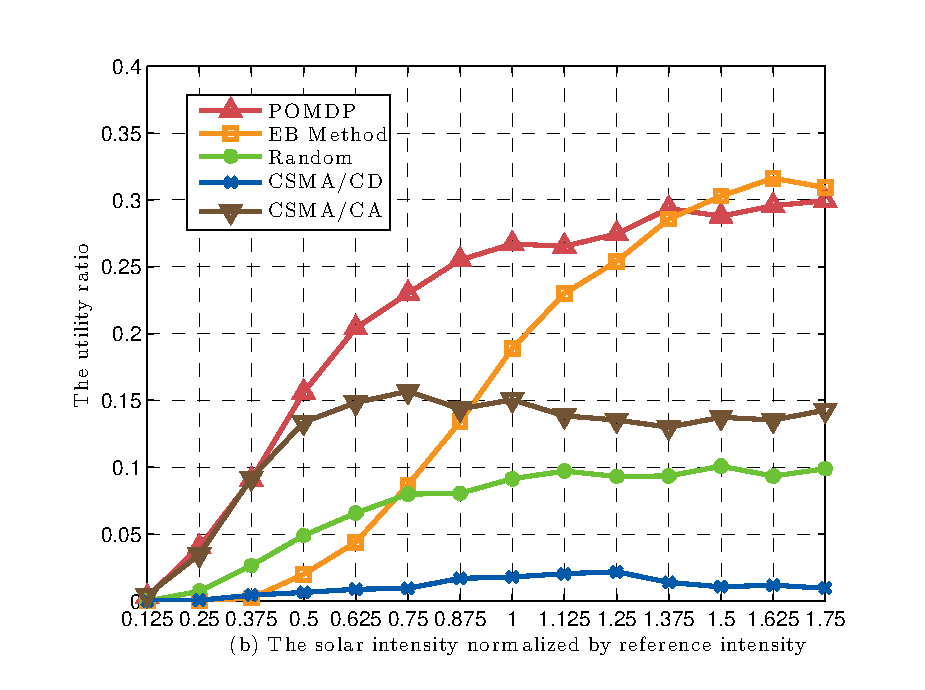
\includegraphics[width=0.5\textwidth]{3_fig1_2.eps}}
\caption{Two BS with \(U_N = 0,\,1,\, N_B = 3\)}
\end{figure}
\indent In Fig. 3, we consider single BS with possible number of user from \(0,\, 1,\, 2,\, 3\), \(N_B = 8\), \(B_M = N_BP_TT_L\),
and the leaving rate \(\mu = 0.05\). 
In Fig. 3 (a), the \(\mu_S = 1\) and \(\sigma_S = 0.5\), and in Fig. 3 (b), the arrival rate \(\lambda = 0.4\). 
As shown in the figure, the performance of proposed POMDP is significantly higher,
with the EM method's overall performance following at the second place,
which validates the efficiency of our algorithms.
From (a), the CSMA/CD method could have a good performance when the system is not busy,
but decreases quickly with the increasing arrival rate of users.
From (b), it is also clear that even when the solar intensity is strong, 
the traditional algorithms' ability to increase utility is still obviously limited.
As they are not able to make use of the EH information of the system.
It is also worth noting that, as we predicted, when the solar intensity is strong,
the suboptimal EB method will approach the proposed POMDP method.\\
\indent In Fig. 4, multiple BSs are considered, with possible number of user from \(0,\, 1,\), \(N_B = 3\), \(B_M = N_BP_TT_L\),
and the leaving rate \(\mu = 0.05\). 
Besides what we find in Fig. 3, we also find in Fig. 4 
that when the possible serving positions is limited, the crowded system make the CSMA/CD method almost useless.
In (b), when the solar intensity is small, the utility of CSMA/CD increases with intensity due to more available sources.
But when the solar intensity is big, 
the more solar intensity, the more users are staying in the BS, 
and thus the CSMA/CD has less chances of being served.
Also, in (b), the suboptimal EB method could overperform POMDP method when the intensity is big, 
which is mainly brought by the errors caused in the POMDP formulation, like using the quasi-static assumption.
\section{Conclusion}
In this paper, we proposed a powerful POMDP algorithm to solve the access problem in EH powered network,
which is promising and instructive in building a national range Super Wi-Fi network.
The framework given in this paper is adjustable to EH problems other than the Solar EH one.
A suboptimal EB method is proposed as well.
The affect of solar intensity, user arriving rate, leaving rate and many other features are considered, 
proving our work reliable and effective.
And the future work of this paper focuses on the adjustment and prediction of system parameters.
\bibliographystyle{IEEEtran}
\bibliography{Ref}
\end{document}
